\documentclass[UTF8]{article}
\usepackage{ctex}
\usepackage{listings}
\usepackage[bf,small,indentafter,pagestyles]{titlesec} 

\usepackage{geometry}  %边距和纸张大小
\geometry{a4paper}
\geometry{left=2cm,right=2cm,top=3cm,bottom=3cm}

\usepackage{fancyhdr}

\usepackage{url}
%\usepackage{graphicx} %使用graphicx包
\usepackage{graphicx}
%\DeclareGraphicsExtensions{.eps,.pdf,.jpg,.png}
%\DeclareGraphicsRule{.jpg}{eps}{.bb}{}
%\DeclareGraphicsRule{.png}{eps}{.bb}{}
%\DeclareGraphicsRule{.pdf}{eps}{.bb}{}


\usepackage{amsmath}
\usepackage{amssymb} %使用数学符号使用 
\usepackage{cite} %使用引用 
\usepackage{enumerate}
%使用item使用

\begin{document} 



\renewcommand{\contentsname}{\center{\huge 目\ \ \ 录}}
%%这个renew需要放在最前面,提前进行定义
\author{    彭峰     05121214   }
 \date{2015-5-10}
\title{忆阻}  %题目要改掉   后面
 \titlespacing{\chapter}{0pt}{*0}{*4}
\titlelabel{\S\thetitle\quad}

\tableofcontents

\maketitle

\section{前言}

先说说选题原因:还记得当年忆阻在实验室真正被实现时,我通过刊物了解到忆阻这一划时代的器件终于从理论转到实验阶段。还记得当时HP公司说希望在2012年实现成品进入市场。当时还很欣喜,说到时候就能用上这么高端的产品了,未想到现在还是处于实验室阶段,还在研究特性中。。

本次的选题实际上还是有极大的偏移的,忆阻作为第四种元件,虽然也可以当作电阻器使用,但也应该和电阻和电容处于同一层次才是。但是想想这样和大家的选题不同,加之之前有过一次邂逅,以前也有过了解,还是决定以“忆阻”为选题方向吧。

\section{背景介绍}
%先是全中文的
1971年华裔科学家蔡少棠提出忆阻的概念,在研究电荷、电流、电压和磁通量之间的关系时,外推了对称的非线性电阻(电压与电流),非线性电容器(电压与电荷),和非线性电感(磁通量与电流)之间的的概念,
他推断在电阻、电容和电感器之外,应该还有一种组件,代表着电荷与磁通量之间的关系。由这张图可以很好地展现四种基本元件的关系。


\begin{figure}[htbp]
\centering
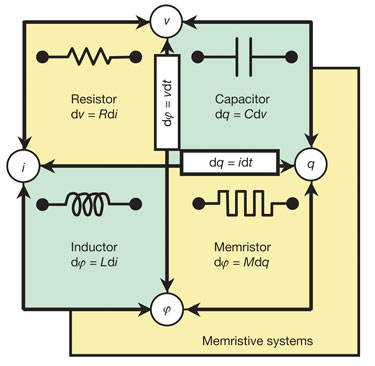
\includegraphics[width=1.77in,height=1.75in]{pic/memristor01.jpeg}
%\caption{This is an inserted JPG graphic}  这个选项需要添加figure后才可用
\caption{四种基本元器件}
\label{fig:3}
\end{figure}



在理论提出之前,蔡少棠发现在电流(i)、电压(v),电荷(q)及磁通量($\phi_{B}$)4种变量之间的6种关系有5种是已知的,从图中我们可以看到,电阻是电压和电流之间的关系,电感是电流和磁通量之间的关系,电容是电压和电荷之间的关系,忆阻理论的提出很好的填补了四种基本物理量关系的空白。
在理论提出的当时,还没有实际的器件,只是在数学模型上忆阻应该存在。%这里找当时原论文的出处

\begin{figure}[htbp]
\centering
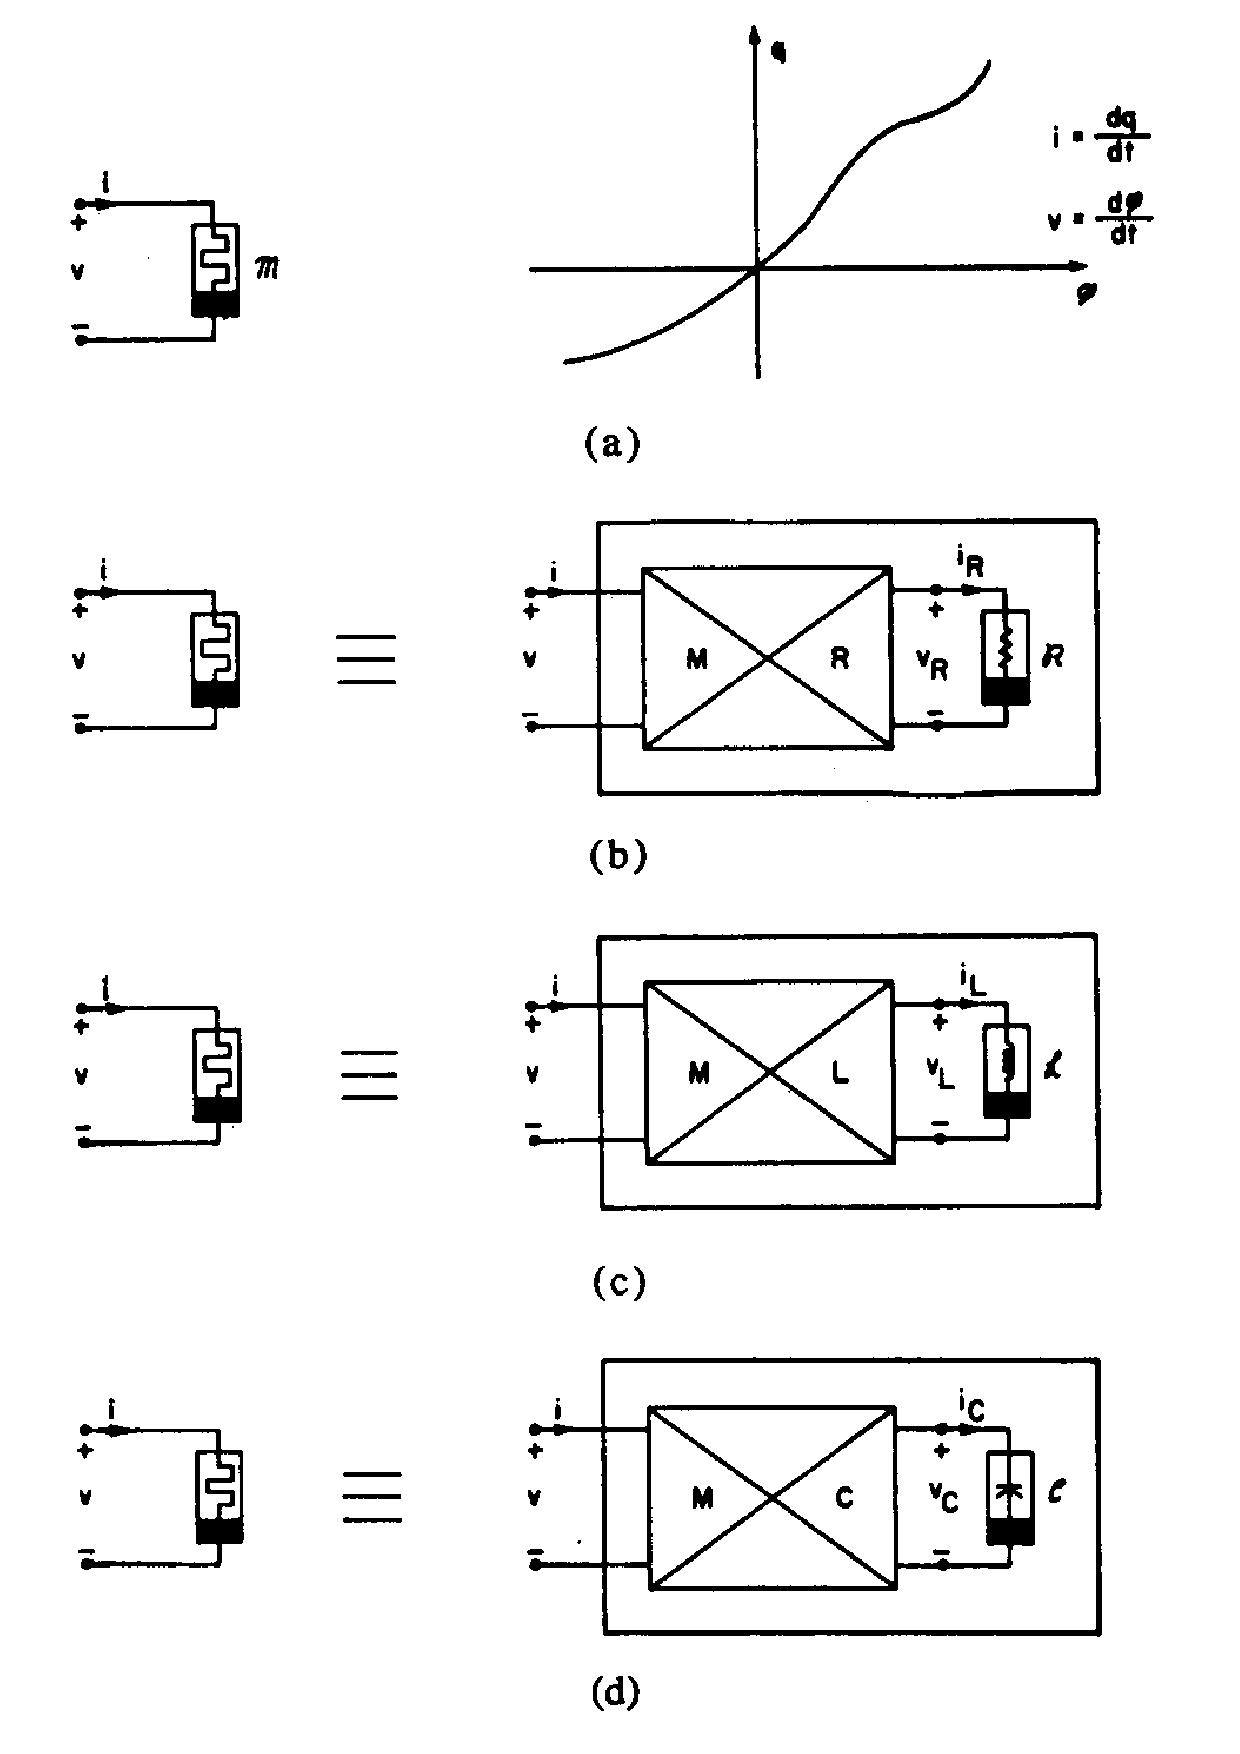
\includegraphics[width=1.77in,height=1.75in]{pic/4}
%\caption{This is an inserted JPG graphic}  这个选项需要添加figure后才可用
\caption{忆阻推论}
\label{fig:4}
\end{figure}



\section{忆阻是如何被发现的}

这一理论可追溯到上世纪90年代末,当时惠普公司高级研究员Stan Williams建立了该公司的信息和量子系统实验室,以便开拓未来20年的计算技术。40年来,工业界不断制造基于摩尔定律的更小、更便宜的晶体管。于是,Williams研究团队开始研发越来越小的晶体管,这致使他们考虑当设备缩小到单个分子大小时会发生什么,以及单个原子运动将如何影响其性能。




在一次试验中,Stanley Williams 的团队发现,一块极薄的二氧化钛被夹在两个电极中间,这
些二氧化钛又被分成两个部份,一半是正常的二氧化钛,另一半进行“掺杂”,使氧原子数减少。因此“掺杂”的那一半带正电,电流通过时电阻比较小,而且当电流从“掺杂”的一边通向正常的一边时,在电场的影响之下缺氧的“掺杂物”会逐渐往正常的一侧游移,使得以整块材料来言,“掺杂”的部份会占比较高的比重,整体的电阻也就会降低。反之,当电流从正常的一侧流向“掺杂”的一侧时,电场会把缺氧的“掺杂物”从回推,电阻就会跟着增加。
\begin{figure}[htbp]
\centering
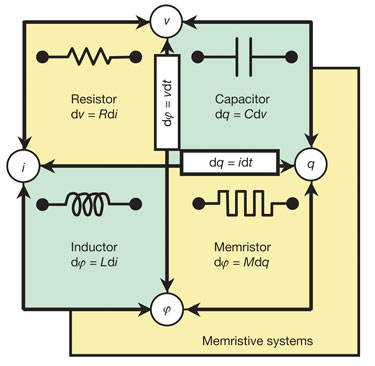
\includegraphics[width=1.77in,height=1.75in]{pic/memristor01.jpeg}

\caption{氧原子流动示意图}
\label{fig:graph}
\end{figure}



%这里以HP公司提出的一个理论模型为例对其进行解释。
,如图示。掺杂了氧空位的氧化钛 层电阻较小,纵横 闩中掺杂层所占比例较大,纵横闩处于导通状态 ;无掺杂氧空 位的氧化钛层 电阻较大,纵横闩中无掺杂层所 占比例较大,纵横闩处于断路状 态。纵横闩的电阻可以简单的看做是掺杂部分 电阻和无掺杂部分的电阻之和。 令纵横闩的总厚度为D,掺杂层的即时厚度为$\mathnormal{w(t)}   $,若纵横闩全部为掺杂层 , 总电阻记为$R_{ON}$ ,那么掺杂层的即时电阻为$R_{ON} \frac{\mathnormal{w_{t}}}{\mathnormal{D}}$。若纵横闩全部为无掺杂 层,总电阻记为$R_{OFF}$ ,无掺杂层的即时电阻为$R_{OFF}(1 - \frac{w_{t}}{D})$。当忆阻器电极施 加偏置电压$v(t)$,忆阻器内部会导致离子迁移。设在理 欧姆接触及线性的 电子迁移的情况下,离子迁移率为$\mu_{\gamma}$
\begin{equation}
v_{t} = (R_{ON} \frac{w_{t}}{D} + R_{OFF}(1 - \frac{w_{t}}{D}) ) i(t)
\end{equation}
\begin{equation}
\frac{dw(t)}{dt} = \mu_{\gamma}\frac{R_{ON}}{D}q(t)
\end{equation}

两式()()很好的满足了忆阻数学特性模型()()

\begin{figure}[htbp]
\centering
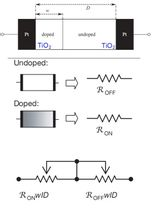
\includegraphics[width=1.77in,height=1.75in]{pic/no2.jpeg}

\caption{等效器件}
\label{fig:graph}
\end{figure}




%%HP团队的研究情况
HP的两个不同团队的研究成果:


%
%+ Crossbar Latch 原理  ----
%Crossbar Latch 的原理是由一排横向和一排纵向的电线组成的网格,在每一个交叉点上,放上一个「开关」连结一条横向和纵向的电线。让这两条电线控制这个开关的状态,使其产生开、关两种状态,这样可以和计算机额的0、1相对应。那网格上的每一个交叉点都能储存一个位的数据。
我们结合实现的一个典型的忆阻做成的开关的图来看:
\begin{figure}[htbp]
\centering
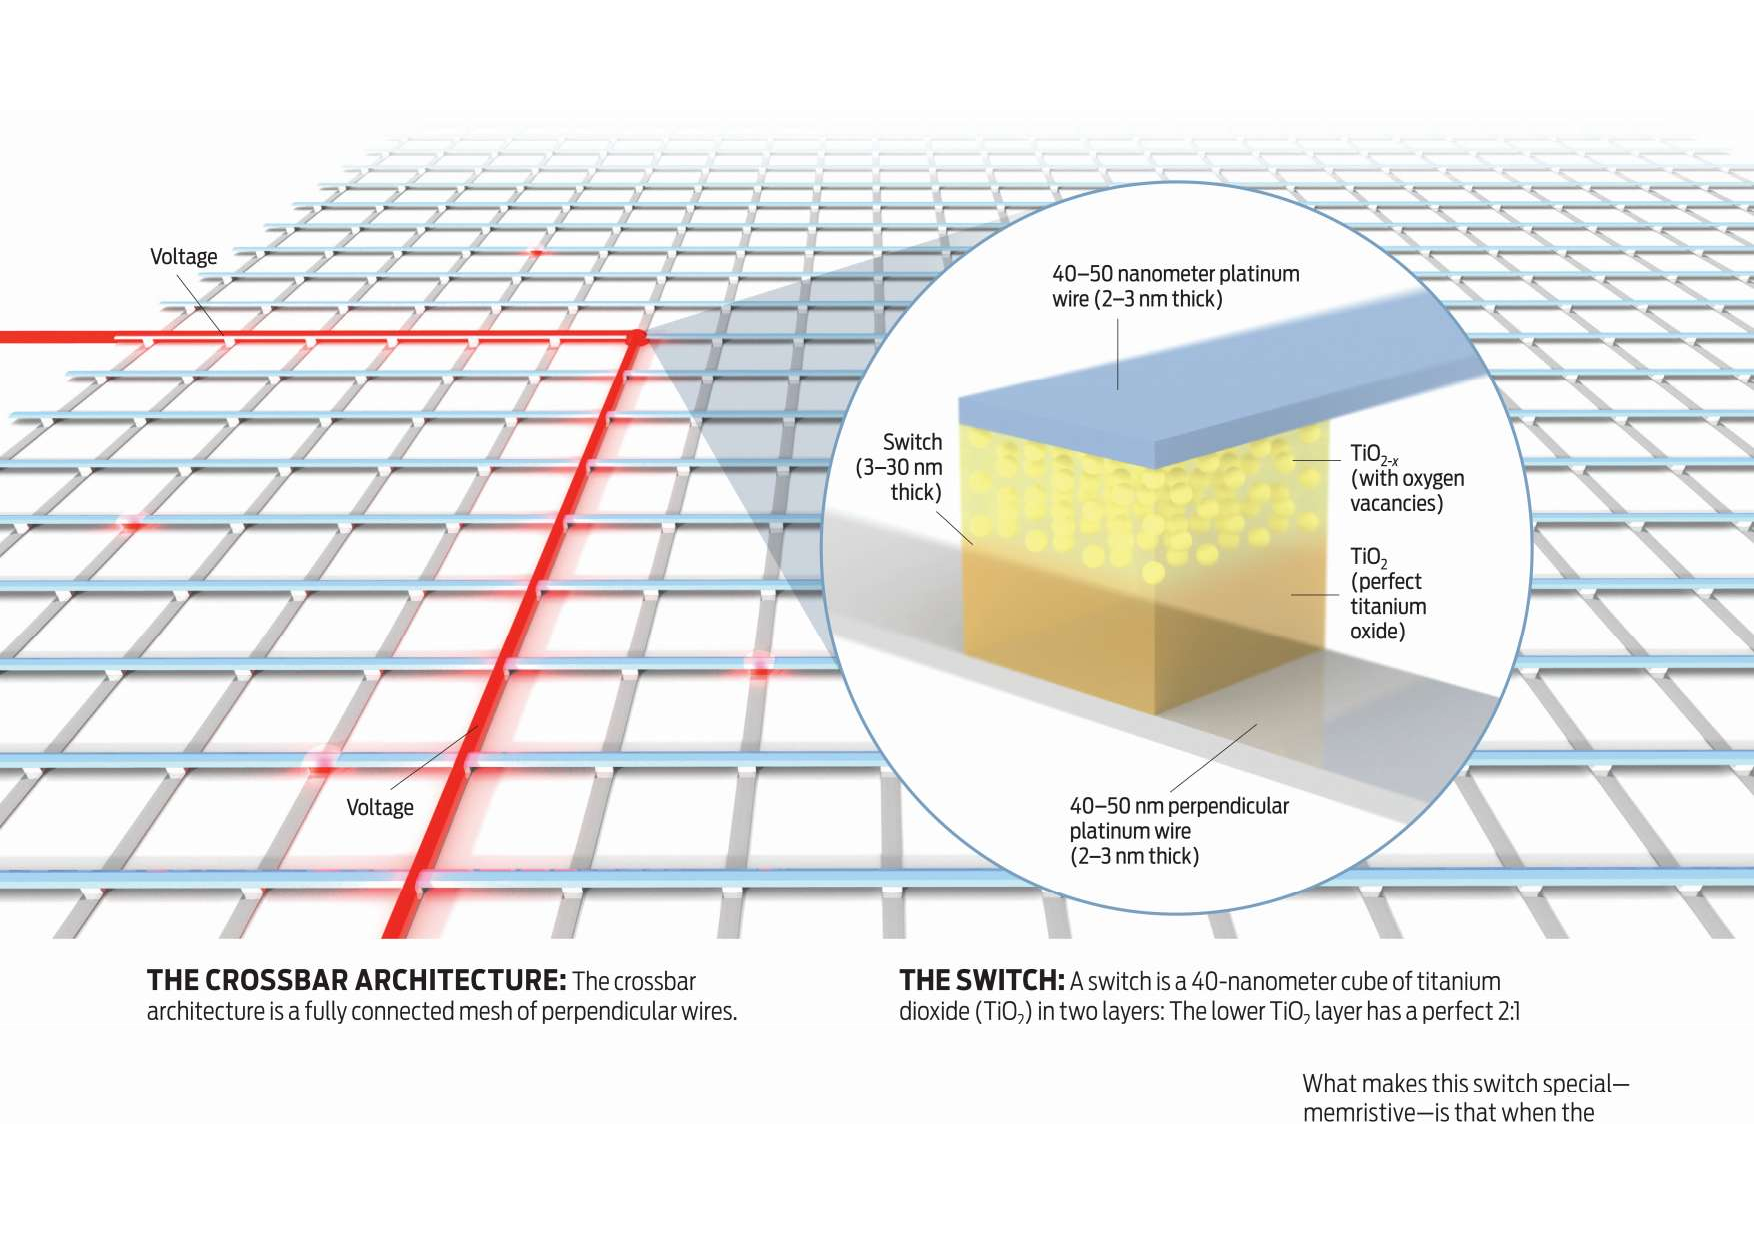
\includegraphics[width=5.77in,height=3.75in]{pic/7}

\caption{忆阻门}
\label{fig:7}
\end{figure}
图中形成一个类似三明治的结构,最上方是纳米级的导线,中间部分是$TiO_{2}$层,内部包含游离的氧原子,下部是$TiO_{3}$层,内部原子结合较为稳定。最下方是又一根纳米数量级导线



%+ Stanley Williams ----二氧化硅当作忆阻器----(带图的)
%%%%下面是性能部分,需要更多的修改



\section{忆阻器的理论和性能}

忆阻器的特性--忆阻值M 满足式\eqref{eq:1}的特性:
\begin{equation}\label{eq:1}
M = \frac{\mathrm d\phi_{B}}{\mathrm dq}
\end{equation}

根据法拉第电磁感应定律及复合函数求导法则.对其积分,有:
\begin{equation}\label{eq:2}
M(q(t)) = \frac{\int\mathnormal{v(t)dt}}{\int\mathnormal{i(t)dt}}
\end{equation}
由式\eqref{eq:2}可以看出,忆阻的值和电阻有着相同的量纲,但是其阻值取决于过去流过的电荷的总量,即忆阻有着记忆特性,且在断电状态下保持不变。这和电容器的电压比较类似。

%R(I)=\frac{\mathrm dV}{\mathrm dI}
我们用一个表格来看下忆阻器的行为:

\begin{tabular}{|c|c|c|}
\hline
& 电荷(q)& 电流(I) \\

 \hline
电压(U)  & 电容(倒数) &电阻率 \\
     & $\frac{1}{C}=\frac{\mathrm{d}U}{\mathrm{d}q}=\frac{\mathrm{d}\dot \Phi}{\mathrm{d}q}$  &   $R=\frac{\mathrm{d}U}{\mathrm{d}I}=\frac{\mathrm{d}\dot \Phi}{\mathrm{d}\dot{q}}$ \\
 \hline
磁通量($\Phi$)  & 忆阻器 & 电感 \\
     & $M=\frac{\mathrm{d}\Phi}{\mathrm{d}q}$  &  $L=\frac{\mathrm{d}\Phi}{\mathrm{d}I}=\frac{\mathrm{d}\Phi}{\mathrm{d}\dot{q}}$ \\
 \hline

\end{tabular}

%%%%%%下面添加一些理论更深的东西,这里先不加,主要看下HP的模型建立,如果没时间的话就下周的周末做啊






\section{一个常见原型}
这里介绍的是HP公司在当时忆阻器件发现之后提出的一种模型。



%\section{工业界发展}  没有工业界,现在还是处于实验室阶段
HP 关于忆阻器的发现在 2008 年时发表于「自然」期刊,2009 年证明了 Cross Latch 的系统很容易就能堆栈,形成立体的内存。这意味着可以每平方英寸能存储的容量极大,加之可以进行堆栈的3D构成,可以见到是存储的一种绝佳替代品。

2012年,HRL实验室(一个由通用汽车公司和波音公司共有的研究设施)宣布首次成功运行忆阻器阵列,即利用了用于电子设备生产的互补金属氧化物半导体(CMOS)制造工艺。

澳大利亚墨尔本皇家理工大学 的科学家用非晶 钙钛矿氧化物开发出一种纳米级超快忆阻器,采用了一种纳米级的薄膜材料来制 造忆阻器 ,这种 功能性氧化物 比人类 头发的直径薄 1 000倍 。这种材料 在化学 上具有 “忆 阻”效应 ,存储 在其 中的数 据具有非易失性 。 



\section{忆阻器的未来}
 同时,如何建造忆阻器的理念也在持续演进。在6月中旬召开的惠普公司探索会议上,该公司首席技术官Martin Fink概述了一个简单的体系结构,他将其简单地称为“机器”。它包含一套记忆电路,并利用光导纤维而非铜线连接到高效专用处理器上。

该行业有若干目标处于变化中。忆阻器可以大大提高电子元件的能源效率,并能更好地处理数据洪流。对于这些设备的发展而言,一个必不可少的因素是,计算能力和储存密度指数式增长的延续,在过去40年里,这些产品的价格出现了暴跌。出于类似原因,IBM刚刚宣布将投入30亿美元,用于研发实验性“后硅”结构和芯片,并预计在10年里能出现现存体系的根本性变化。

这些变化将带来计算机操作系统的极大变化,以适应不再区分动态存储器和长期存储的计算机硬件。Bresniker认为这种改变是一个契机,以抛弃烦琐的操作系统代码——这些代码以前用来适应老式硬件的限制。

%%%%%
“我们开发出的这种忆阻器在电子 ? 设备中具有广泛的应用价值,无论是能收缩到纳米 j 尺度 的超快存储设备 ,还是基于计算机逻辑体系架 I 构的生物神经网络存储器。‘未来这种忆阻器将能够 j 替代目前所广泛使用的闪存、固态硬盘,让电子设备 j 更快、更轻、使用时间更长。虽然目前还有很多的研 ! 究需要做,但已经能够肯定的是,新发现为寻找下一代内存设备,构建复杂的神经网络图形 ; 


\end{document}
